\chapter{Optically amplified detection for biomedical sensing and imaging}
\label{chp:JOSAA2013_Chapter}

Optical sensing and imaging methods for biomedical applications such as spectroscopy and laser-scanning fluorescence microscopy are incapable of performing sensitive detection at high scan rates due to the fundamental trade-off between sensitivity and speed. This is because fewer photons are detected during short integration times and hence the signal falls below the detector noise. Optical postamplification can, however, overcome this challenge by amplifying the collected optical signal after collection and before photodetection. Here we present a theoretical analysis of the sensitivity of high-speed biomedical sensing and imaging systems enhanced by optical postamplifiers. As a case study, we focus on Raman amplifiers because they produce gain at any wavelength within the gain medium's transparency window and are hence suitable for biomedical applications. Our analytical model shows that when limited by detector noise, such optically postamplified systems can achieve a sensitivity improvement of up to 20 dB in the visible to near-infrared spectral range without sacrificing speed. This analysis is expected to be valuable for design of fast real-time biomedical sensing and imaging systems.

\section{Introduction} \label{sec:JOSAA2013_Section1}

Fast real-time optical sensing and imaging are essential tools for studying fast transient processes in biomedical applications such as neuroscience \cite{ohki2005functional,golshani2009internally}, laser surgery \cite{slade2000complete}, and extracorporeal shockwaves \cite{delius2002twenty,riehle1987principles}. They are equally important for microfluidic biotechnology applications (e.g., flow cytometry) \cite{goda2009serial,squires2005microfluidics,watson2004introduction} that require high-throughput analysis of a large population of cells and pathogens with minimum error. Another important application is Raman spectroscopy in which high-speed sensing capability is needed to investigate fast chemical changes such as those that occur during combustion \cite{hult2007high} and chemical reactions between biological molecules \cite{epstein1998introduction,petty2006spatiotemporal,siesler2008near}. Some examples of applications that require both high scan rates and high detection sensitivity are laser-scanning confocal microscopy, fluorescence microscopy, coherent anti-Stokes Raman spectroscopy, and two-photon microscopy used to observe neural activity in real time \cite{diaspro2001confocal}. Here even higher throughput is desirable to monitor the dynamics of a large number of neurons simultaneously.
The central requirement for these studies is a signal integration time that is much shorter than the time scale of dynamic processes. This requirement must be satisfied, but is difficult to meet due to the fundamental trade-off between sensitivity (minimum detectable power) and speed; at high scan rates, fewer photons are detected during the short integration time within each scan period. This leads to the loss of sensitivity in high-speed detection as it is limited by detector noise (typically thermal noise in the photodetector).

The reduced sensitivity can be compensated for by the use of high-intensity illumination, which, in fact, is frequently used in industrial applications. However, this approach is not suitable for biomedical applications as it can damage the biological sample. The problem becomes much more severe in microscopy because focusing the light onto the sample with an objective lens results in an extremely high intensity. Another technique used to reduce detector thermal noise is detector cooling. However, this is undesirable as it requires a refrigeration unit to accompany the detector and hence adds significant cost and complexity to the detector design and reduces reliability.

Optical postamplification (after signal collection and before photon-to-electron conversion) can circumvent this fundamental challenge when the detection sensitivity is limited by detector noise (typically thermal noise) \cite{goda2009serial,goda2008amplified,mahjoubfar2011high,goda2009theory,tsia2010performance,qian2009real,han2003photonic,goda2013dispersive}. It eliminates the need for high-intensity illumination and cooling and represents a novel method for detecting weak optical signals in biomedical sensing and imaging applications. As shown in Figure \ref{fig:JOSAA2013_Figure1}, an optical postamplifier before the photodetector increases the optical signal while the detector thermal noise is intact and hence improves the sensitivity of the detection system in the thermal noise limited region, which is the case in high-speed sensing and imaging. Unlike detector cooling, optical postamplification can be easily employed before photodetection to improve the sensitivity with no need for modifications of the detector design. 

\begin{figure}[htb!]
\centering
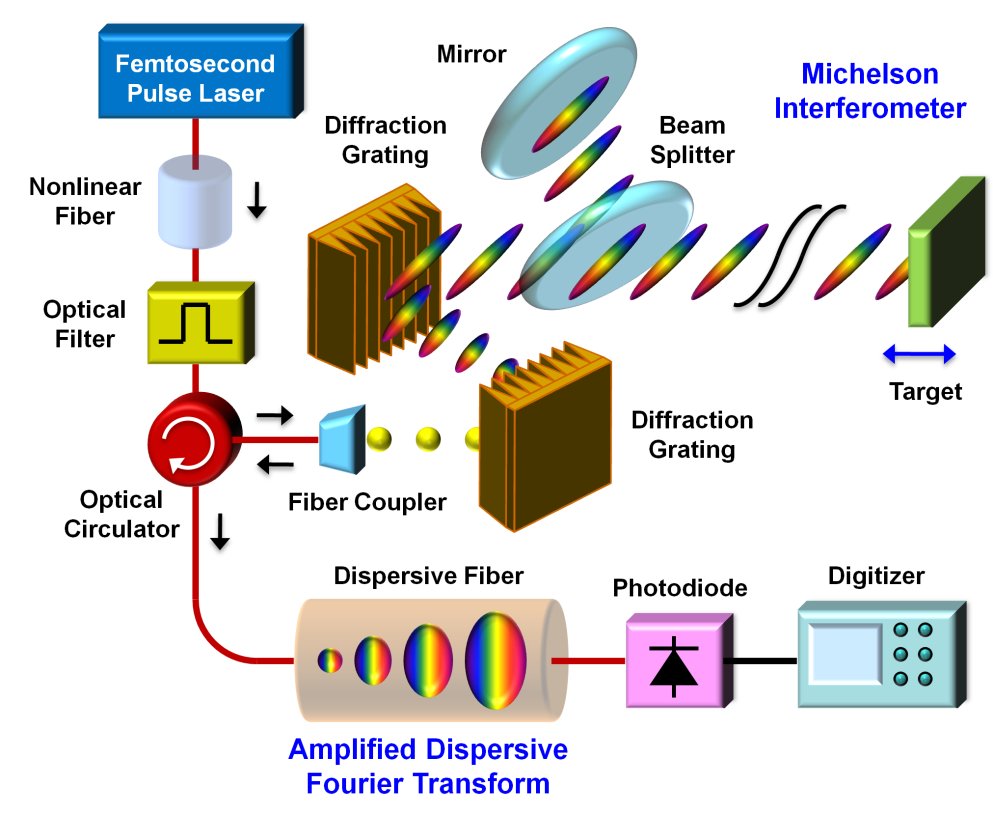
\includegraphics[scale=0.85]{JOSAA2013/Figure1.png}
\caption{Detector sensitivity improvement by an optical postamplifier in high-speed detection. (a) (i) The optical signal is buried in the thermal noise of the photodetector (ii) whereas an optical postamplifier increases the optical signal with the thermal noise intact resulting in an improvement in the sensitivity of the detection system. (b) Comparison of the signal-to-noise ratios for photodetection (i) with and (ii) without an optical postamplifier shows that the optical postamplifier is useful when the detection sensitivity is thermal noise limited because the signal-to-noise ratio is directly proportional to the square of the collected optical power. Here, the signal-to-noise ratio and the collected optical power are both in logarithmic scale. ASE-ASE: amplified spontaneous emission self-beat; ASE-S: amplified spontaneous emission -- signal beat; RIN: relative intensity noise; DRB: double Rayleigh backscattering. (These noise components are detailed in Section \ref{sec:JOSAA2013_Section3}.).}
\label{fig:JOSAA2013_Figure1}
\end{figure}

Optical postamplification is fundamentally different from the use of electronic signal intensifiers [e.g. micro-channel plates used in photomultiplier tubes (PMTs) or intensified charge-coupled device (ICCDs)] in that amplification occurs in the optical domain whereas in electronic signal intensifiers, it occurs in the electronic domain. Electronic signal intensifiers are complex vacuum tube devices that require high voltage sources. Also, their scan rates are limited by the fundamental trade-off between gain and bandwidth in all electronic systems \cite{horowitz1989art}. While PMTs are extremely sensitive detectors useful for capturing faint light or even counting single photons, they are unsuitable for continuous high-speed detection due to the limited bandwidth and the dead time caused by their gated operation.

Among different approaches to optical amplification, stimulated Raman scattering (SRS) \cite{agrawal2007nonlinear,islam2002raman} provides several advantages over other methods such as rare-earth doped fiber amplifiers and semiconductor optical amplifiers (SOAs). First, gain is possible at any wavelength as long as a pump is available at a frequency blue-shifted from the signal by the optical-phonon vibrational frequency \cite{agrawal2007nonlinear}. Second, a broad and flexible gain spectrum can be obtained by using multiple pump fields \cite{islam2002raman}. Finally, Raman amplifiers have a lower noise figure than rare-earth doped fiber amplifiers and SOAs \cite{islam2002raman,goda2009demonstration}. For these reasons, Raman amplifiers are routinely employed in fiber-optic communication \cite{islam2002raman}.

Recently, we have reported Raman amplification of a weak optical signal in a single-mode fiber in the 800 nm spectral range for the first time \cite{goda2009demonstration,mahjoubfar2010raman}. This proof-of-principle demonstration has shown potential utility of Raman amplifiers to biomedical sensing and imaging applications. While noise sources associated with Raman amplifiers have been extensively studied in the fiber-optic communication band (1300 - 1600 nm), virtually no such work has been done in the optical spectrum outside of the fiber-optic communication band. However, the short wavelength band (500 - 900 nm) is important for biomedical applications as most of them are conducted in this band in favor of low water absorption and high spatial resolution in imaging.

In this chapter, we theoretically analyze the sensitivity of a detection system enhanced by a Raman fiber amplifier as an optical postamplifier at such short wavelengths. This postamplifier can be easily used in fiber-based biomedical imaging and sensing devices such as fiber-coupled confocal and fluorescence scanning microscopes \cite{bird2002compact,kimura1991confocal}, serial time-encoded microscopes \cite{goda2009serial,tsia2010performance,goda2012hybrid,mahjoubfar2013label}, and fiber-optic biosensors \cite{wolfbeis2004fiber,song2006refractive,piliarik2003surface}. However, it is impractical to employ this fiber amplifier before a free-space imaging or sensing system e.g. a charge-coupled device (CCD) or a complementary metal--oxide--semiconductor (CMOS) image sensor because the fiber coupling losses mostly defeat the benefits of the postamplification. First, we review the basic concept of the Raman amplifier in Section \ref{sec:JOSAA2013_Section2}. We then derive the variances of noise photocurrents associated with the Raman amplifier as well as photodetection in Section \ref{sec:JOSAA2013_Section3}. With the results in Section \ref{sec:JOSAA2013_Section3}, we evaluate and compare the noise current variances and then study the sensitivity of the detection system enhanced by the amplifier in Section \ref{sec:JOSAA2013_Section4}. We also perform numerical simulations to obtain a set of parameter values that optimize the performance of the detection system at various wavelengths. In Section \ref{sec:JOSAA2013_Section5}, we conclude this chapter.

\section{Raman amplification as an optical postamplifier} \label{sec:JOSAA2013_Section2}

Raman amplification is an optical process based on the phenomenon of SRS \cite{agrawal2007nonlinear,islam2002raman}. As shown in Figure \ref{fig:JOSAA2013_Figure2}, in SRS an input field (called the Stokes field) stimulates the inelastic scattering of a blue-shifted pump field inside an optical medium mediated by its vibrational modes (called optical phonons). As with the rare-earth doped fiber amplifiers, Raman amplifiers based on the process of Raman amplification are often used to increase optical signals in fiber-optic communications with transmission fibers as gain media \cite{agrawal2007nonlinear,islam2002raman}.

A typical Raman amplifier is schematically shown in Figure \ref{fig:JOSAA2013_Figure2}. It consists of a single-mode silica fiber as a gain medium, an input weak field (Stokes field), and one or two continuous-wave pump fields that couple into and out of the fiber via duplexers such as fiber-based wavelength-division multiplexers or dichroic beamsplitters in free space. In many cases, the fiber is bidirectionally pumped in the forward and backward directions to optimize the performance of the amplifier.

\begin{figure}[htb!]
\centering
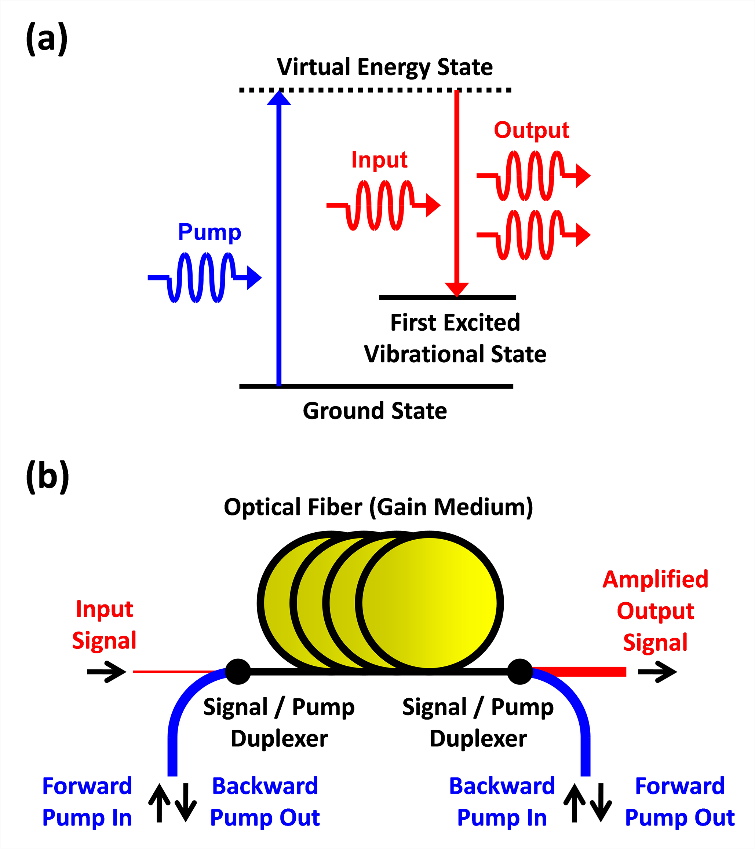
\includegraphics[scale=1]{JOSAA2013/Figure2.png}
\caption{Energy diagram of stimulated Raman scattering (SRS) and basic schematic of a SRS-based optical postamplifier. (a) Raman amplification is an optical process based on the phenomenon of SRS in which the input field (called the Stokes field) stimulates the inelastic scattering of a blue-shifted pump field inside an optical medium mediated by its vibrational modes (optical phonons). (b) A typical Raman amplifier consists of a single-mode silica fiber (gain medium), an input at the Stokes frequency, and one or two pump fields that couple into and out of the fiber via duplexers such as wavelength-division multiplexers or dichroic beamsplitters. The fiber is bidirectionally pumped in the forward and backward directions to optimize the performance of the amplifier.}
\label{fig:JOSAA2013_Figure2}
\end{figure}

Raman amplification in an optical fiber is governed by the following coupled equations:
\begin{eqnarray}
\frac{\ud I_s}{\ud z} &=& g_R I_p I_s - \alpha_s I_s,\label{eqn:JOSAA_Equation_1}\\
\frac{\ud I_p}{\ud z} &=& -\frac{\omega_p}{\omega_s} g_R I_p I_s- \alpha_p I_p,\label{eqn:JOSAA_Equation_2}
\end{eqnarray}
where $I_s$ and $I_p$ are the intensities of the Stokes and pump fields, respectively, $\omega_s$ and $\omega_p$ are the optical frequencies of the Stokes and pump fields, respectively, $\alpha_s$ and $\alpha_p$ are the loss coefficients of the fiber at the Stokes and pump frequencies, respectively, $g_R$ is the Raman gain coefficient, and $z$ is the propagation distance.

Assuming that the pump field is much more powerful than the input signal (which is often the case) and hence undepleted, the first term on the right hand side in Equation \eqref{eqn:JOSAA_Equation_2} can be ignored and the pump intensity decreases exponentially in the fiber. If the fiber is bidirectionally pumped, the total pump intensity at an arbitrary position in the fiber can be obtained from Equation \eqref{eqn:JOSAA_Equation_2} and is given by
\begin{equation}
I_p(z) = I_p^f(z) + I_p^b(z),\label{eqn:JOSAA_Equation_3}
\end{equation}
where 
\begin{eqnarray}
I_p^f(z) &=& I_p^f(0) \mathrm{e}^{-\alpha_p z},\label{eqn:JOSAA_Equation_4a}\\
I_p^b(z) &=& I_p^b(L) \mathrm{e}^{-\alpha_p (L-z)}.\label{eqn:JOSAA_Equation_4b}
\end{eqnarray}
Here $L$ is the total length of the fiber, $I_p^f(0)$ and $I_p^b(L)$ are the intensities of the forward and backward pump fields at fiber ends, respectively, which can be obtained from the pump powers in the forward and backward directions,
\begin{eqnarray}
I_p^f(0) &=& \frac{P_p^f(0)}{\pi(d_p/2)^2},\label{eqn:JOSAA_Equation_5a}\\
I_p^b(L) &=& \frac{P_p^b(L)}{\pi(d_p/2)^2},\label{eqn:JOSAA_Equation_5b}
\end{eqnarray}
where $P_p^f(0)$ and $P_p^b(L)$ are the forward and backward pump powers, respectively, and $d_p$ is the mode field diameter of the pump fields in the fiber. Likewise, the Stokes intensity can also be obtained from the input power (Stokes power),
\begin{equation}
I_s(z) = \frac{P_s(z)}{\pi(d_s/2)^2},\label{eqn:JOSAA_Equation_6}
\end{equation}
where $d_s$ is the mode field diameter of the Stokes field in the fiber. Here we have assumed that the forward and backward pump fields are uncorrelated and do not interfere with each other in the fiber.
Substituting Equation \eqref{eqn:JOSAA_Equation_3} into Equation \eqref{eqn:JOSAA_Equation_1}, the intensity of the Stokes field at an arbitrary point in the fiber, $I_s(z)$, can be obtained, and hence, the net gain is also found to be
\begin{equation}
G(z)=\frac{I_s(z)}{I_s(0)}=\exp\left\{\frac{g_R}{\alpha_p} \left[I_{p}^f(0)\left(1-\mathrm{e}^{-\alpha_p z}\right)+I_{p}^b(L)\left(\mathrm{e}^{-\alpha_p (L-z)}-\mathrm{e}^{-\alpha_p L}\right)\right]- \alpha_s z\right\},\label{eqn:JOSAA_Equation_7}
\end{equation}
where $I_s(0)$ is the intensity of the input Stokes field before entering the fiber.

\section{Limiting noise sources} \label{sec:JOSAA2013_Section3}

In order to evaluate the performance of the Raman amplifier, or more specifically, to study the sensitivity of a detection system enhanced by the amplifier, it is important to understand limiting noise sources associated with the amplifier. In this section, we derive analytical forms for such noise components. We then evaluate and compare them using realistic parameter values in the next section.

\subsection{Double Rayleigh backscattering noise}

Rayleigh scattering is the elastic scattering of light by particles (i.e., atoms and molecules) with dimensions which are much smaller than the wavelength of the light. Rayleigh scattering by molecules in the fiber medium (typically glass) is a fundamental loss mechanism in all optical fibers. While most of the scattered light escapes through the cladding, a small portion of the light can stay in the fiber core and propagate backward in the fiber. This backward-propagating scattered light is normally very weak, but it can be amplified by distributed Raman amplification in the fiber. The amplified backward-propagating scattered light can again be scattered and propagate along with the signal in the forward direction. This causes a delayed crosstalk in-band noise that is amplified by the process of SRS in the fiber \cite{agrawal1997fiber,kim2002reflection}. It is called double Rayleigh backscattering (DRB) noise \cite{islam2004raman,lewis2000characterization} and is known to play a critical role in limiting the performance of Raman amplifiers in long-haul fiber-optic communication systems \cite{hansen1998rayleigh}.

The crosstalk-to-signal ratio or fraction of the signal power that is scattered by DRB and amplified is given by \cite{nissov1999rayleigh}
\begin{equation}
f_{DRB} = r_s^2 \int_0^L G^{-2}(z) \int_z^L{G^2(z') \ud z'} \ud z,\label{eqn:JOSAA_Equation_8}
\end{equation}
where $r_s$ is the Rayleigh baskscattering coefficient. Since this is proportional to the Rayleigh scattering loss, it is inversely proportional to $\lambda_s^4$, where $\lambda_s$ is the wavelength of the input (Stokes) field. Therefore, the DRB noise is an important limiting noise factor at shorter (visible) wavelengths used in biomedical applications than in the fiber-optic communication links because they operate in the longer-wavelength infrared band.

The variance of the DRB noise photocurrent produced by the photodiode is given by \cite{headley2005raman}
\begin{equation}
\left\langle \delta i_{DRB}^2\right\rangle = 2 f_{DRB} [r_d G(L) P_s(0)]^2,\label{eqn:JOSAA_Equation_9}
\end{equation}
where $r_d$ is the responsivity of the photodetector, and $P_s(0)$ is the input Stokes power. The factor of 2 in the equation accounts for the two polarization modes of the fiber.

\subsection{Pump-to-Stokes relative intensity noise transfer}

Every laser including pump lasers in Raman amplifiers has intensity fluctuations called relative intensity noise (RIN) which typically originate from laser cavity vibration, instability in the laser gain medium (caused by the feedback between electron and photon populations), or transferred intensity noise from a pump source. As the Raman amplifier is powered by one or more pump fields, their RIN can transfer to the amplified (Stokes) signal through the process of SRS.

Using the RIN calculation technique described for a singly-pumped Raman amplifier in Ref. \cite{fludger2001pump}, the transfer function of the pump RIN to the Stokes RIN in bidirectionally pumped Raman amplifiers is found to be
\begin{eqnarray}
&&\hspace{-1.7cm}RIN_s(f) = \nonumber\\
&&\hspace{-1.5cm}\left\{\frac{v_s\left[\alpha_s L + \ln G(L)\right]}{L_{eff}}\right\}^2 \nonumber\\
&&\hspace{-1.5cm}\left\{RIN_p^f(f) \left[\frac{P_p^f(0)}{P_p^f(0)+P_p^b(L)}\right]^2 \left[\frac{1-2\mathrm{e}^{-\alpha_p L}\cos(bfL/v_s)+\mathrm{e}^{-2 \alpha_p L}}{(\alpha_p v_s)^2+(b f)^2}\right] \right.\nonumber\\
&&\hspace{-1.5cm} \left.+RIN_p^b(f) \left[\frac{P_p^b(L)}{P_p^f(0)+P_p^b(L)}\right]^2 \left[\frac{1-2\mathrm{e}^{-\alpha_p L}\cos(4 \pi f L/v_s)+\mathrm{e}^{-2 \alpha_p L}}{(\alpha_p v_s)^2+(4 \pi f)^2}\right]\right\}, \label{eqn:JOSAA_Equation_10}
\end{eqnarray}
where $f$ is the electrical frequency of the detection circuitry (also called the sideband frequency of the optical carrier), $RIN_p^f(f)$ and $RIN_p^b(f)$ are the RIN coefficient of the forward and backward pump lasers, respectively, $v_s$ is the group velocity of the Stokes field, $L_{eff}$ is the effective length of the fiber at the pump wavelength and is given by
\begin{equation}
L_{eff}=\frac{1-\exp(-\alpha_p L)}{\alpha_p},\label{eqn:JOSAA_Equation_11}
\end{equation}
and a constant, $b$, is defined in terms of the difference in group velocity between the pump and Stokes fields by
\begin{equation}
b = 2\pi\left(1-\frac{v_s}{v_p}\right).\label{eqn:JOSAA_Equation_12}
\end{equation}
Here $v_p$ is the group velocity of the pump fields. The first and second terms in Equation \eqref{eqn:JOSAA_Equation_10} account for the RIN transfer from the forward and backward pump RINs to the Stokes RIN, respectively.

The variance of the RIN transfer noise photocurrent produced by the photodiode is found by integrating the beat between the Stokes field and the pump-RIN-transferred Stokes noise over the electrical bandwidth of the photodetector, $B_e$, to be
\begin{equation}
\left\langle \delta i_{RIN}^2\right\rangle = \int_0^{B_e}RIN_s(f) [r_d G(L) P_s(0)]^2 \ud f.\label{eqn:JOSAA_Equation_13}
\end{equation}

\subsection{Amplified spontaneous emission noise}

When an optical gain medium is pumped to produce population inversion (hence gain), the random spontaneously emitted light is amplified by the process of stimulated emission. This process is called amplified spontaneous emission (ASE) and produces photons that have random phases relative to the signal and appear as noise. The SRS-induced ASE noise gives rise to two beat-noise signals that appear at baseband frequencies: (1) beating of the Stokes field with the ASE and (2) beating of the ASE with itself. The variances of these noise photocurrents generated at the photodiode are given by \cite{headley2005raman,agrawal2001applications}
\begin{eqnarray}
\left\langle \delta i_{s-ASE}^2\right\rangle &=& 4 r_d^2 G(L) P_s(0) S_{ASE} B_e, \label{eqn:JOSAA_Equation_14}\\
\left\langle \delta i_{ASE-ASE}^2\right\rangle &=& 4 r_d^2 S_{ASE}^2 B_e \left(B_o-\frac{B_e}{2}\right), \label{eqn:JOSAA_Equation_15}
\end{eqnarray}
where $B_o$ is the optical bandwidth of the photodetector, $B_e$ is the electrical bandwidth of the detection system ($B_e$ is assumed to be $< B_o/2$), and $S_{ASE}$ is the spectral density of the ASE defined by \cite{kogelnik1964considerations}
\begin{equation}
S_{ASE} = n_{sp} \hbar \omega_s g_R G(L) \int_0^L {\frac{I_p(z)}{G(z)} dz}.\label{eqn:JOSAA_Equation_16}
\end{equation}
Here $\hbar$ is the reduced Planck constant, and $n_{sp}$ is the population inversion factor given by
\begin{equation}
n_{sp}=\left\{1-\exp\left[-\frac{\hbar (\omega_p-\omega_s)}{k_B T_f}\right]\right\}^{-1},\label{eqn:JOSAA_Equation_17}
\end{equation}
where $k_B$ is the Boltzmann constant, and $T_f$ is the temperature of the gain medium i.e. optical fiber. In Equations \eqref{eqn:JOSAA_Equation_14} and \eqref{eqn:JOSAA_Equation_15}, the factor of 4 comes from the beating of two fields having two polarization modes. Equation \eqref{eqn:JOSAA_Equation_16} indicates that $S_{ASE}$ is white and exists at all frequencies within the gain spectrum of the Raman amplifier. Hence, the effect of the ASE on the Stokes field can be reduced by narrowing the optical bandwidth with an optical filter.

\subsection{Detection noise}

For a high-quality detector, the performance of the photodetector circuit is limited by thermal noise from thermal fluctuations in the load resistor, shot noise from the photocurrent, dark (leakage) current noise from the photodiode, and flicker noise. The flicker noise (also called $1/f$ noise) is inversely proportional to the measurement frequency and hence ignored in high-speed detection.

Thermal noise (also called Johnson-Nyquist noise) is the electronic noise produced by the thermal agitation of the electrons inside the load resistor. Thermal noise is approximately white, and hence, its power spectral density is constant throughout the entire detection bandwidth. The variance of the Norton-equivalent thermal noise photocurrent is given by
\begin{equation}
\left\langle \delta i_{thermal}^2\right\rangle = \frac{4 k_B T_d B_e}{R_L},\label{eqn:JOSAA_Equation_18}
\end{equation}
where $T_d$ is the temperature of the photodetector, and $R_L$ is the matched-load resistance of the photodetector circuit.

Shot noise originates from the fluctuations of the number of detected photons and is a direct consequence of the quantum nature of light. Shot noise follows a Poisson distribution and is translated into the variance of the shot noise photocurrent through the photodiode,
\begin{equation}
\left\langle \delta i_{shot}^2\right\rangle = 2 q r_d G(L) P_s(0) B_e,\label{eqn:JOSAA_Equation_19}
\end{equation}
where $q$ is the elementary charge. Similar to thermal noise, shot noise is also white with constant power spectral density throughout the detection bandwidth.

Dark current is the relatively small electric current that flows through the photodiode when it is not exposed to light. It is due to the random generation of free carriers within the depletion region of the photodiode. The variance of the dark noise photocurrent through the photodiode is given by
\begin{equation}
\left\langle \delta i_{dark}^2\right\rangle = 2 q \left\langle i_{dark}\right\rangle B_e,\label{eqn:JOSAA_Equation_20}
\end{equation}
where $\left\langle i_{dark}\right\rangle$ is the average dark current of the photodiode. The total noise variance of the photodetector is given by the sum of Equations \eqref{eqn:JOSAA_Equation_18}, \eqref{eqn:JOSAA_Equation_19}, and \eqref{eqn:JOSAA_Equation_20}.

\section{Sensitivity analysis} \label{sec:JOSAA2013_Section4}

In the last section, we have derived the noise photocurrent variance of different noise components for an optically postamplified detection system. In this section, we evaluate and compare these at 800 nm using realistic parameter values to determine the detection sensitivity. Finally, we investigate sensitivity improvements offered by the optical amplifier at wavelengths other than 800 nm.

\subsection{Comparison of various noise components}

To evaluate the noise photocurrent variances derived in the last section, we use realistic values for the parameters listed in Tables \ref{tbl:JOSAA2013_Table1_part1} and \ref{tbl:JOSAA2013_Table1_part2}. For the Raman amplifier, we first choose the Stokes wavelength to be 800 nm because we previously reported the experimental demonstration of Raman gain at this wavelength \cite{goda2009demonstration, mahjoubfar2010raman}. To maximize the Raman gain in fused silica fibers, the Stokes frequency shift should be about 13 THz \cite{islam2002raman}, which corresponds to the pump wavelength of 773.2 nm for the Stokes wavelength of 800 nm. Also, the 3-dB Raman gain bandwidth of fused silica fibers is more than 5 THz \cite{islam2002raman}, resulting in an amplifier bandwidth of over 10 nm centered at 800 nm. If a larger bandwidth is required, multiple pump lasers at different wavelengths over the gain spectrum can be used \cite{islam2002raman}. The Raman gain coefficient at $\lambda_s$ = 800 nm can be estimated from \cite{rottwitt2003scaling}
\begin{equation}
g_R(\lambda_s)=\frac{\Lambda_s}{\lambda_s}\frac{A_{eff}(\Lambda_s)}{A_{eff}(\lambda_s)}g_R(\Lambda_s),\label{eqn:JOSAA_Equation_21}
\end{equation}
where $g_R(\Lambda_s)$ is the Raman gain coefficient at a reference wavelength, $\Lambda_s$, and $A_{eff}$ is the average mode field diameter between the pump and Stokes fields and is given by $A_{eff}=[\pi(d_s/2)^2+\pi(d_p/2)^2]/2$ evaluated at each wavelength. Using the well-known Raman gain coefficient of $g_R(\Lambda_s)= 6 \times 10^{-14}$ m/W at $\Lambda_s = 1500$ nm for silica fibers \cite{islam2002raman}, the Raman gain coefficient is found to be $g_R(\lambda_s) =  4.57 \times 10^{-13}$ m/W.
The fiber attenuation of typical fibers at the Stokes and pump wavelengths are 2.31 dB/km and 2.66 dB/km, respectively, which correspond to the fiber loss coefficients of $5.32 \times 10^{-4}$ m$^{-1}$ and $6.13 \times 10^{-4}$ m$^{-1}$, respectively. The input power of the forward and backward pump fields and the fiber length are chosen to be both 200 mW and 1040 m, respectively. Our analysis shows that this combination of pump powers and fiber length maximizes the sensitivity enhancement. A shorter fiber length can be chosen for the Raman amplifier, but it requires higher pump powers to maintain the same gain.

\begin{table}[t]
\begin{centering}
\begin{tabular}{|c|c|c|c|} \hline
Name & Parameter & Unit & Value\\ \hline\hline
Reduced Planck Constant & $\hbar$ & J$\cdot$s & $1.05457 \times 10^{-34}$ \\ \hline
Boltzmann Constant & $k_B$ & J/K & $1.38065 \times 10^{-23}$  \\ \hline
Elementary Charge & $q$ & C & $1.60218 \times 10^{-19}$  \\ \hline 
Stokes Wavelength & $\lambda_s$ & nm & 800 \\ \hline
Pump Wavelength & $\lambda_p$ & nm & 773.2 \\ \hline
Fiber Attenuation at Stokes & $\alpha_s$ & m$^{-1}$ & $5.32 \times 10^{-4}$ \\ \hline
Fiber Attenuation at Pump & $\alpha_p$ & m$^{-1}$ & $6.12 \times 10^{-4}$ \\ \hline
Raman Gain Coefficient & $g_R$ & m/W & $4.57 \times 10^{-13}$ \\ \hline
Group Velocity at Stokes & $v_s$ & m/s & $2.053373 \times 10^8$ \\ \hline
Group Velocity at Pump & $v_p$ & m/s & $2.052073 \times 10^8$ \\ \hline
Mode Field Diameter at Stokes & $d_s$ & $\mu$m & 5.52 \\ \hline
Mode Field Diameter at Pump & $d_p$ & $\mu$m & 5.34 \\ \hline
Fiber Length & $L$ & m & 1040 \\ \hline
Temperature of Fiber& $T_f$ & K & 300 \\ \hline
Rayleigh Backscattering Coefficient & $r_s$ & km$^{-1}$ & $1.41 \times 10^{-3}$ \\ \hline
\end{tabular}
\caption{Parameter values used to evaluate the power of different noise components (continued at Table \ref{tbl:JOSAA2013_Table1_part2}).}
\label{tbl:JOSAA2013_Table1_part1}
\end{centering}
\end{table}

\begin{table}[t]
\begin{centering}
\begin{tabular}{|c|c|c|c|} \hline
Name & Parameter & Unit & Value\\ \hline\hline
Forward Input Pump Power & $P_p^f(0)$ & mW & 200 \\ \hline
Backward Input Pump Power & $P_p^b(L)$ & mW & 200 \\ \hline
Forward Pump Relative Intensity Noise & $RIN_p^f$ & Hz$^{-1}$ & $10^{-13}$ \\ \hline
Backward Pump Relative Intensity Noise & $RIN_p^b$ & Hz$^{-1}$ & $10^{-13}$ \\ \hline
Photodiode Responsivity & $r_d$ & A/W & 0.5 \\ \hline
Photodiode Dark Current & $\left\langle i_{dark}\right\rangle$ & nA & 20 \\ \hline
Matched-load Resistance & $R_L$ & $\Omega$ & 50\\ \hline
Temperature of Photodetector & $T_d$ & K & 300 \\ \hline
Optical Bandwidth of Photodetector & $B_o$ & THz & 0.5 \\ \hline
Electrical Bandwidth of Photodetector & $B_e$ & MHz & 100 \\ \hline
Avalanche Photodiode Gain & $M$ & dB & 10 \\ \hline
Avalanche Photodiode Excess Noise Factor & $F$ & dB & 5 \\ \hline
\end{tabular}
\caption{Parameter values used to evaluate the power of different noise components (continued from Table \ref{tbl:JOSAA2013_Table1_part1}).}
\label{tbl:JOSAA2013_Table1_part2}
\end{centering}
\end{table}

For the DRB noise, the value of the Rayleigh backscattering coefficient, $r_s$, is required. Since the value is about $10^{-4}$ km$^{-1}$ for telecommunication fibers in the 1550 nm spectral band, the coefficient at 800 nm can be estimated to be  $r_s \simeq (1550/800)^4 \times 10^{-4} = 1.41 \times 10^{-3}$ km$^{-1}$. This estimate is based on the $\lambda^{-4}$ behavior of Rayleigh scattering.

For the pump-to-Stokes RIN transfer, given the typical pump RIN noise of 0.1\% over a bandwidth of 10 MHz, the RIN of the forward and backward pump fields is found to be $RIN_p^f = RIN_p^b = (0.1\%)^2/(\SI{10}{MHz}) = 10^{-13}$ Hz$^{-1}$. The group velocities at the Stokes and pump wavelengths are estimated from the Sellmeier equation to be $2.051968 \times 10^8$ m/s and $2.053373 \times 10^8$ m/s, respectively.

For the noise photocurrents associated with the photodetector, the responsivity and dark current of a typical Si photodiode at 800 nm are 0.5 A/W and 20 nA, respectively. The standard load impedance of the photodetector circuit is 50 $\Omega$. The optical and electrical bandwidths of the photodetector are assumed to be 0.5 THz and 100 MHz, respectively. From a noise point of view, a narrow bandwidth is desired. However, in practice, the bandwidth is set by the scan rate of the sensing or imaging system.

Using Equations \eqref{eqn:JOSAA_Equation_9}, \eqref{eqn:JOSAA_Equation_13}, \eqref{eqn:JOSAA_Equation_14}, \eqref{eqn:JOSAA_Equation_15}, \eqref{eqn:JOSAA_Equation_18}, \eqref{eqn:JOSAA_Equation_19}, and \eqref{eqn:JOSAA_Equation_20} and the parameter values in Tables \ref{tbl:JOSAA2013_Table1_part1} and \ref{tbl:JOSAA2013_Table1_part2}, the value (variance) of each noise component is evaluated and shown in Figure \ref{fig:JOSAA2013_Figure3}. The dark current noise, the thermal noise, and the ASE-ASE beat noise are independent of the input signal power. The ASE-signal beat noise and the shot noise are linearly proportional to the input signal power whereas the RIN and the DRB noise are quadratically proportional to the input signal power. Therefore, the ASE-ASE beat noise and the thermal noise are dominant at low input powers while the RIN and the DRB noise are significant at high input powers.

\begin{figure}[htb!]
\centering
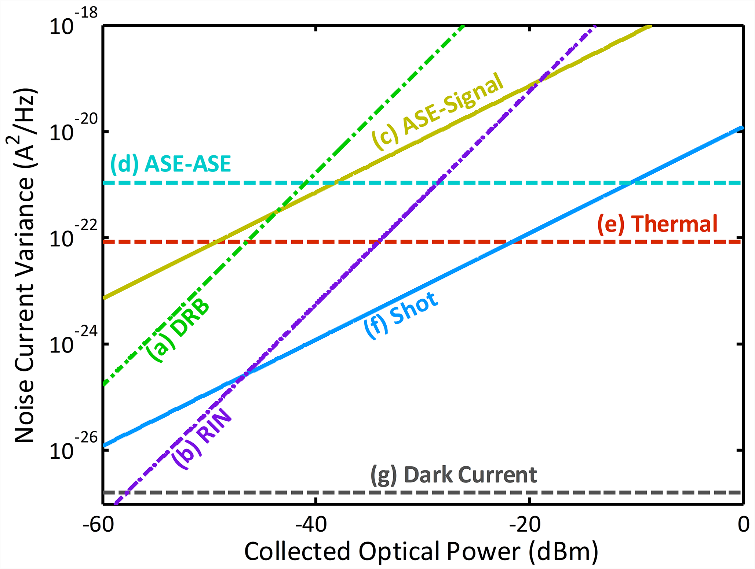
\includegraphics[scale=1]{JOSAA2013/Figure3.png}
\caption{Noise photocurrent variance per 1 Hz detection bandwidth versus the input power to the optical postamplifier (collected optical power). (a) DRB noise, (b) pump-to-Stokes RIN transfer, (c) ASE-signal beat noise, (d) ASE-ASE beat noise, (e) thermal noise, (f) shot noise, and (g) dark current noise. The ASE-ASE beat noise and the thermal noise are dominant at low input powers while the RIN and DRB noise are significant at high input powers.}
\label{fig:JOSAA2013_Figure3}
\end{figure}

\subsection{Signal-to-noise ratio of the detection system enhanced by the Raman amplifier}

The signal-to-noise ratio (SNR) of a detection system with a positive--intrinsic--negative (PIN) photodiode and a Raman fiber postamplifier is given by the power of the signal photocurrent over the total noise current variance,
\begin{equation}
{SNR} = \frac{i_s^2}{\left\langle \delta i_{total}^2\right\rangle}=\frac{[r_d G(L) P_s(0)]^2}{\left\langle \delta i_{total}^2\right\rangle},\label{eqn:JOSAA_Equation_22}
\end{equation}
where the total noise current variance is the sum of all the noise current variances in Equations \eqref{eqn:JOSAA_Equation_9}, \eqref{eqn:JOSAA_Equation_13}, \eqref{eqn:JOSAA_Equation_14}, \eqref{eqn:JOSAA_Equation_15}, \eqref{eqn:JOSAA_Equation_18}, \eqref{eqn:JOSAA_Equation_19}, and \eqref{eqn:JOSAA_Equation_20} such that
\begin{eqnarray}
\left\langle \delta i_{total}^2\right\rangle &=&\left\langle \delta i_{DRB}^2\right\rangle+\left\langle \delta i_{RIN}^2\right\rangle+\left\langle \delta i_{s-ASE}^2\right\rangle+\left\langle \delta i_{ASE-ASE}^2\right\rangle \nonumber\\
&&+\left\langle \delta i_{thermal}^2\right\rangle+\left\langle \delta i_{shot}^2\right\rangle+\left\langle \delta i_{dark}^2\right\rangle.\label{eqn:JOSAA_Equation_23}
\end{eqnarray}
Also, for an avalanche photodiode (APD) the photocurrent is multiplied by a gain factor, $M$, and due to the stochastic nature of the avalanche process, dark and shot noise current variances increase by a factor of $M^2 \cdot F$, where $F$ is excess noise factor of an APD.

Figure \ref{fig:JOSAA2013_Figure4} shows the SNR of the detection system in various detector configurations, indicating an improvement in detection sensitivity by the use of the optical postamplifier after photons are collected and before photodetection. Given an electrical bandwidth of 100 MHz, the postamplifier improves the sensitivity of the PIN photodiode detection system by 19.4 dB compared to the same detection system without the postamplifier. The APD has a sensitivity 10.3 dB higher than the PIN photodiode. However, the combination of the optical postamplifier and PIN photodiode is better in SNR than APD alone by 9.1 dB. Note that the combination of the optical postamplifier and APD does not improve the sensitivity significantly (only 6.1 dB) because the internal gain of the APD is meant to overcome the thermal noise of the detector -- the same function performed by the optical postamplifier, but the APD is not as effective in improving the SNR. The behavior seen in Figure \ref{fig:JOSAA2013_Figure4} is in agreement with the conceptual depiction of SNR dependecy on the input optical power in Figure \ref{fig:JOSAA2013_Figure1}.

\begin{figure}[htb!]
\centering
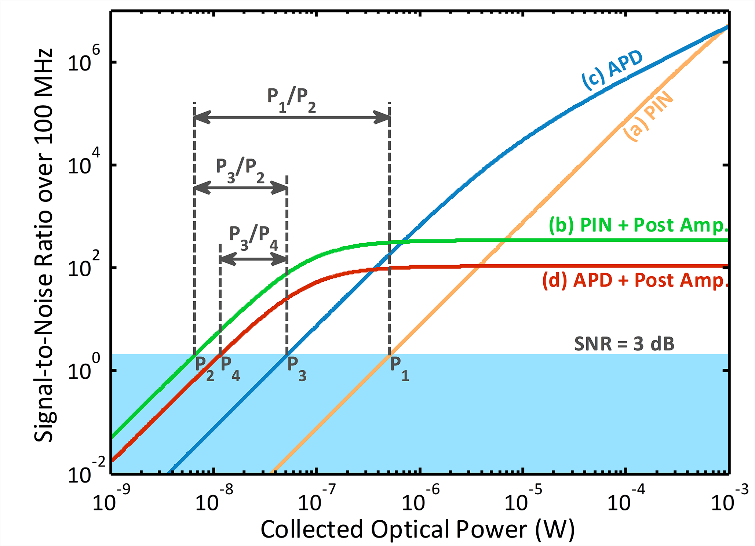
\includegraphics[scale=1]{JOSAA2013/Figure4.png}
\caption{SNR over 100 MHz bandwidth for various detection methods. (a) a positive--intrinsic--negative (PIN) photodiode without a postamplifier, (b) a PIN photodiode with a postamplifier, (c) an avalanche photodiode (APD) without a postamplifier, and (d) an APD with a postamplifier. Comparing (a) and (b), the use of the postamplifier improves the sensitivity of the photodiode detection system by $P_1/P_2 = 19.4$ dB. Comparing (b) and (c), the combination of the postamplifier and the photodiode is better in sensitivity than an APD alone by $P_3 / P_2 = 9.1$ dB.}
\label{fig:JOSAA2013_Figure4}
\end{figure}

\subsection{Sensitivity improvements by the Raman amplifier at various wavelengths}

So far we have focused on the Stokes wavelength of 800 nm. Here we extend the analysis performed at 800 nm to other wavelengths in the visible to near-infrared spectrum where most biological imaging experiments are conducted.

Table \ref{tbl:JOSAA2013_Table2} shows the results of sensitivity improvements with optimized postamplifiers at wavelengths from 500 nm to 1000 nm. To recap, $P_1$ is detection sensitivity of the PIN photodiode without the postamplifier; $P_2$ is detection sensitivity of the PIN photodiode with the postamplifier; $P_3$ is detection sensitivity of the APD without the postamplifier; $P_4$ is detection sensitivity of the APD with the postamplifier; $P_1/P_2$ is sensitivity improvement by the postamplifier for the PIN photodiode; $P_3/P_4$ is sensitivity improvement by the postamplifier for the APD; $P_1/P_3$ is sensitivity advantage of APD over PIN photodiode without any postamplifier; $P_3/P_2$ is sensitivity advantage of the PIN photodiode with the postamplifier over the APD without the postamplifier; $P_4/P_2$is sensitivity advantage of the PIN photodiode with the postamplifier over the APD with the postamplifier.

Postamplifiers are designed to achieve maximum sensitivity improvement at each Stokes wavelength by optimal choice of fiber length and pump powers. It can be seen that at all these wavelengths, the sensitivity of a photodiode with the optical postamplifier, $P_2$, is about two orders of magnitude better than the sensitivity of a photodiode without one, $P_1$ . Note that in the amplifier-enhanced detection system, the degree of the sensitivity enhancement, $P_1/P_2$, improves as the input wavelength increases. Also, the sensitivity, $P_2$, enhances at longer Stokes wavelengths. Due to the large Raman gain coefficients at shorter wavelengths, comparably short fibers and pump lasers with relatively small powers are sufficient to reach the optimum sensitivity improvements. At 500 nm, a fiber of only 100 m is required to reach the optimum sensitivity improvement. The slight increase in the required pump power at 500 nm is due to the complicated interplay of the DRB noise, ASE-signal beat noise, and ASE-ASE beat noise.

\begin{table}[t]
\begin{centering}
\begin{tabular}{|c|c|c|c|c|c|c|c|} \hline
Parameter & Unit & \multicolumn{6}{|c|}{Values at Different Wavelengths} \\ \hline\hline
$\lambda_s$ & nm & 500 & 600 & 700 & 800 & 900 & 1000 \\ \hline
$\lambda_p$ & nm & 489.4 & 584.8 & 679.4 & 773.2 & 866.2 & 958.4 \\ \hline
$d_s$ & $\mu$m & 3.5 & 4.2 & 4.9 & 5.5 & 6.2 & 6.9 \\ \hline
$d_p$ & $\mu$m & 3.4 & 4.1 & 4.7 & 5.3 & 6.0 & 6.6 \\ \hline
$g_R$ & pm/W & 1.79 & 1.06 & 0.674 & 0.457 & 0.324 & 0.238 \\ \hline
$P_p^f(0)$ &mW & 200 & 175 & 175 & 200 & 250 & 400 \\ \hline
$P_p^b(L)$ &mW & 200 & 175 & 175 & 200 & 250 & 400 \\ \hline
$L$ &m & 100 & 270 & 610 & 1040 & 1420 & 1360 \\ \hline
$P_1$ &nW  & 533.67 & 533.67 & 533.67 & 533.67 & 533.67 & 533.67 \\ \hline
$P_2$ &nW  & 9.33 & 8.11 & 7.05 & 6.14 & 5.34 & 4.64 \\ \hline
$P_3$ &nW  & 49.77 & 49.77 & 49.77 & 49.77 & 49.77 & 49.77 \\ \hline
$P_4$ &nW  & 18.7 & 14.2 & 12.3 & 12.3 & 10.7 & 9.33 \\ \hline
$P_1/P_2$ &dB & 17.6 & 18.2 & 18.8 & 19.4 & 20.0 & 20.6 \\ \hline
$P_3/P_4$ &dB  & 4.2 & 5.5 & 6.1 & 6.1 & 6.7 & 7.3 \\ \hline
$P_1/P_3$ &dB & 10.3 & 10.3 & 10.3 & 10.3 & 10.3 & 10.3 \\ \hline
$P_3/P_2$ &dB  & 7.3 & 7.9 & 8.5 & 9.1 & 9.7 & 10.3 \\ \hline
$P_4/P_2$ &dB  & 3.1 & 2.4 & 2.4 & 3.0 & 3.0 & 3.0 \\ \hline
\end{tabular}
\caption{Predicted detection sensitivity and sensitivity improvement at various wavelengths.}
\label{tbl:JOSAA2013_Table2}
\end{centering}
\end{table}
 
As shown in Figure \ref{fig:JOSAA2013_Figure5}, further analysis of the sensitivity and the sensitivity improvement indicates that they reach the optimum levels at certain pump powers beyond which they cannot be improved any more because DRB noise limiting region has reached. At these wavelengths, the maximum sensitivity improvement ranges from 17 to 21 dB. The same maximum sensitivity can be achieved with shorter fibers, but requires higher pump powers to maintain the same Raman gain. Note that better sensitivities (lower minimum detectable powers) and higher sensitivity improvements are achievable at lower pump powers with the input signal at shorter wavelengths while better optimum sensitivities and sensitivity improvements can be obtained at longer Stokes wavelengths.


\begin{figure}[htb!]
\centering
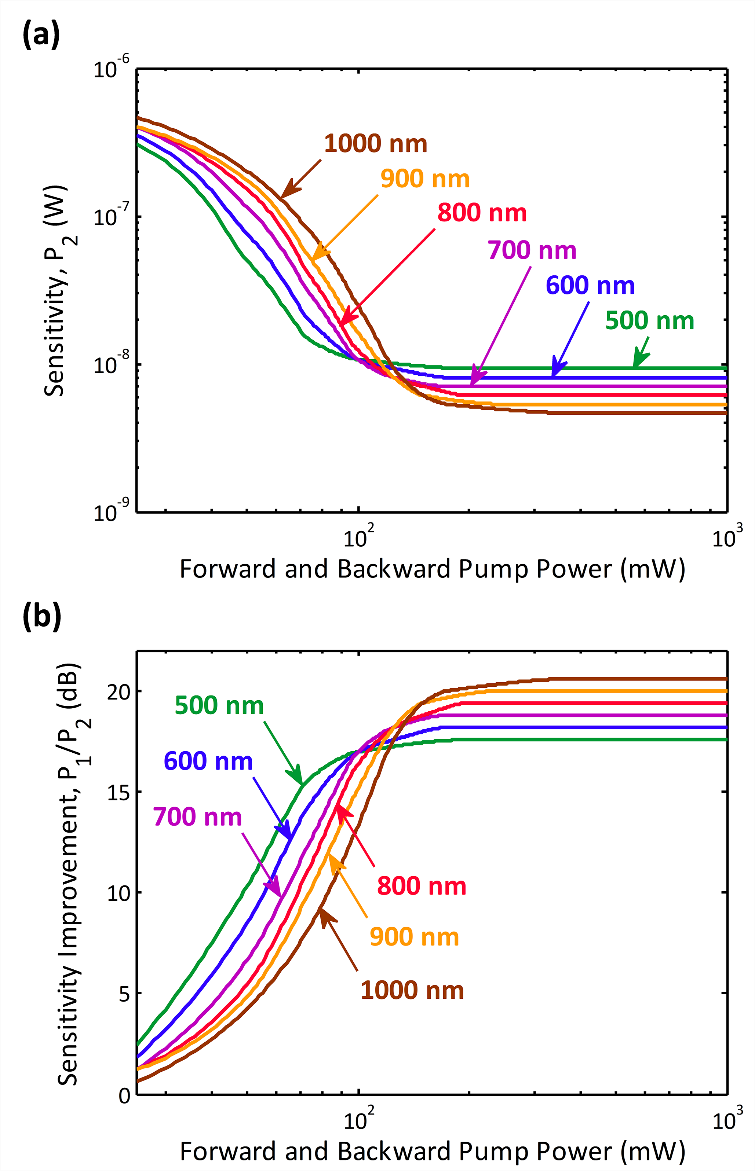
\includegraphics[scale=1]{JOSAA2013/Figure5.png}
\caption{Predicted detection enhancement by optical postamplification over 100 MHz bandwidth in the visible to near-infrared spectral range. (a) Amplifier-enhanced sensitivity (minimum detectable power of the input signal) at various input wavelengths. (b) Sensitivity improvements by the postamplifier for a photodiode at various input wavelengths. Note that better sensitivities (lower minimum detectable powers) and higher sensitivity improvements are achievable at lower pump powers with the input signal at shorter wavelengths while better optimum sensitivities and sensitivity improvements can be obtained at longer input wavelengths.}
\label{fig:JOSAA2013_Figure5}
\end{figure}

\section{Conclusion} \label{sec:JOSAA2013_Section5}

In summary, we have shown that the use of an optical postamplifier can improve the sensitivity of a high-speed photodetection system in the visible to near-infrared spectral range. To analyze the sensitivity of the detection system with a Raman postamplifier, we have derived and compared various noise photocurrents. More specifically, we have demonstrated a sensitivity improvement of about 20 dB in the amplifier-enhanced detection system at Stokes wavelengths from 500 to 1000 nm using a 100 MHz bandwidth which supports very high scan rates. This analysis is expected to be valuable for design of optical postamplifiers for high-speed detection in biomedical sensing and imaging applications, which cannot tolerate high-intensity illumination.
